\chapter{Κατασκευή}


Η επιλογή ενός συστήματος κατασκευής αρχέτυπων κατασκευών με ευκολία και
ευελιξία στην τροποποίηση της υλοποίησης καθώς αυτές αναπτύσσονται και
προκύπτουν νέα απαιτήσεις και προβλήματα.

%Επιθυμητό είναι η ύπαρξη έτοιμων λύσεων σε συνήθεις απαιτήσεις τέτοιων συστημάτων ??
Στοιχεία από CNC.
\\

ΑΝΑΦΟΡΑ ΓΕΝΙΚΑ (με σχετική απεικόνιση) ότι υπάρχει μία κινητή μονάδα μετρήσεων
(για να έχει ο αναγνώστης κατά νου τι επιχειρείται)
%WHY OPEN FRAME?
%λειτουργική μονάδα

%\subsection{Οδηγοί}
\section{Οδηγοί}

Το βασικότερο δομικό στοιχείο είναι το VSlot, εφεξής οδηγός, το οποίο
χρησιμοποιείται τόσο για την κατασκευή του σκελετού όσο και για γραμμική κίνηση,
επιτρέποντας οποιοδήποτε τμήμα της κατασκευής να χρησιμοποιηθεί ως φορέας
κινητών φορτίων.

Οι οδηγοί διαθέτουν αυλακώσεις οι οποίες, επικλινείς στο ανώτερο τμήμα,
χρησιμοποιούνται ως διάδρομοι τροχών και ως υποδοχείς ιμάντα, καλωδίων ή άλλων
συνδετικών εξαρτημάτων στο κατώτερο τμήμα.
Στο σχήμα \ref{fig:construct:vslot} παρατίθεται η μορφή των τεσσάρων διαθέσιμων
μεγεθών οδηγών.
Κατασκευάζονται σε μήκος 1 και 1.5m από κράμα αλουμινίου 6063-T5 -- μέταλλο
μαλακό -- το οποίο επιτρέπει την εύκολη αναπροσαρμογή του μήκους τους.

\begin{figure}
    \caption{Τα τέσσερα μεγέθη οδηγών V-Slot.
    \label{fig:construct:vslot}}
    \begin{center}%
    \def\svgwidth{0.8\textwidth}
%    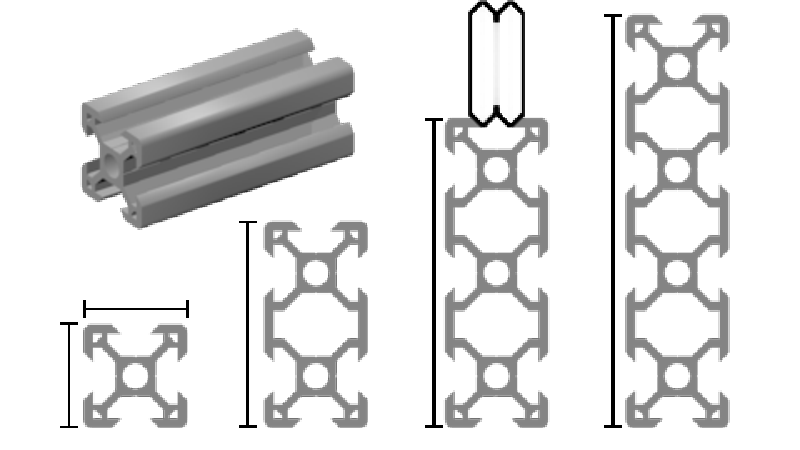
\includegraphics[width=0.7\textwidth]{construct_vslot.png}%
    \input{img/construct_vslot.pdf_tex}
    \end{center}

    Αρχέτυπο σχέδιο:
\end{figure}

%\subsection{Τροχοί}
\section{Τροχοί}

Συντίθενται από ανεξάρτητα μέρη, με αυτόν τον τρόπο επιτρέποντας την προσαρμογή
τους στις απαιτήσεις κάθε περίπτωσης, την αντικατάσταση κάποιου πιθανού
ελαττωματικού μέρους αντί ολόκληρου του τροχού καθώς και πιθανές μελλοντικές
επεκτάσεις της κατασκευής τους.
Το επίσωτρο των τροχών διαθέτει, σαφώς, συμβατή μορφή με τις αυλακώσεις των
οδηγών και εφάπτεται στο ανώτερο τμήμα των αυλακώσεων δίχως να εισέρχεται πλήρως
μέσα σε αυτές ώστε να αποφεύγονται φθορές στον τροχό κατά την κίνησή του από την
επαφή του με τα τοιχώματα.
%Στην εσωτερική κοιλότητα του επίσωτρου τοποθετείται, εφαρμοστά, ζεύγος ένσφαιρων
%τριβέων για τη μείωση των τριβών μεταξύ του τροχού και του άξονα περιστροφής.
%Στο σχήμα \ref{fig:construct:wheel_exploded} παρατίθενται τα μέρη που συνθέτουν
%έναν υποδειγματικό τροχό· βίδα M5, διαχωριστικό, ένσφαιρος τριβέας, επίσωτρο,
%δακτύλιος, δεύτερος ένσφαιρος τριβέας, αντιπερικόχλιο. Ο λόγος ύπαρξης του
%έκκεντρου διαχωριστικού (eccentric spacer) αιτιολογείται σε επόμενη παράγραφο.
% ως άξονας περιστροφής και για την πρόσδεση του τροχού

Στο σχήμα \ref{fig:construct:wheel_exploded} παρατίθενται τα μέρη που συνθέτουν
έναν υποδειγματικό τροχό, και, συνοπτικά περιγράφονται παρακάτω:
\begin{flushleft}
\begin{description}
    \item[Βίδα M5 (α)] ως άξονας περιστροφής και για την στερέωση του τροχού.
    \item[Διαχωριστικό (β)] για την κάλυψη της απόστασης μέχρι την αυλάκωση.
    \item[Έκκεντρο διαχωριστικό (γ)] ως εναλλακτικό του απλού διαχωριστικού. Η
    χρήση αυτού αντί του απλού διαχωριστικού περιγράφεται σε επόμενη παράγραφο.
    \item[Ένσφαιροι τριβείς (δ)] για την μείωση των τριβών μεταξύ τροχού και
    άξονα περιστροφής.
    \item[Επίσωτρο (ε)] για την επαφή με την αυλάκωση.
    \item[Δακτύλιος (στ)] ενδιάμεσος των τριβέων, για την αποφυγή συμπλοκής
    τους.
    \item[Αντιπερικόχλιο (ζ)] για τη συγκράτηση του τροχού στον άξονα.
\end{description}
\end{flushleft}

\begin{figure}
    \caption{Μέλη που αποτελούν τον τροχό.\label{fig:construct:wheel_exploded}}
    \begin{center}%
    \def\svgwidth{0.8\textwidth}
    \input{img/construct_wheel_exploded.pdf_tex}
    \end{center}
    Αρχέτυπο σχέδιο:
\end{figure}

Οι τροχοί στερεώνονται απευθείας στις αυλακώσεις κάποιου οδηγού δίνοντάς του τη
δυνατότητα κύλισης ή σε ξεχωριστή διάτρητη πλάκα η οποία μπορεί να φιλοξενήσει
και πληθώρα άλλων εξαρτημάτων. Η βασικότερη πλάκα είναι η Universal Gantry
Plate, εφεξής πλάκα γεφυρώματος, το αρχέτυπο της οποίας απεικονίζεται στο σχήμα
\ref{fig:construct:gantry-plate}. Οι περισσότερες κυκλικές οπές της είναι
διαμέτρου 5mm ενώ οι επιμήκεις μπορούν να χρησιμοποιηθούν για την πρόσδεση
ιμάντων.

\begin{figure}
    \caption[Πλάκα γεφυρώματος]{Πλάκα γεφυρώματος (μονάδες σε mm).
    \label{fig:construct:gantry-plate}}
    \begin{center}%
    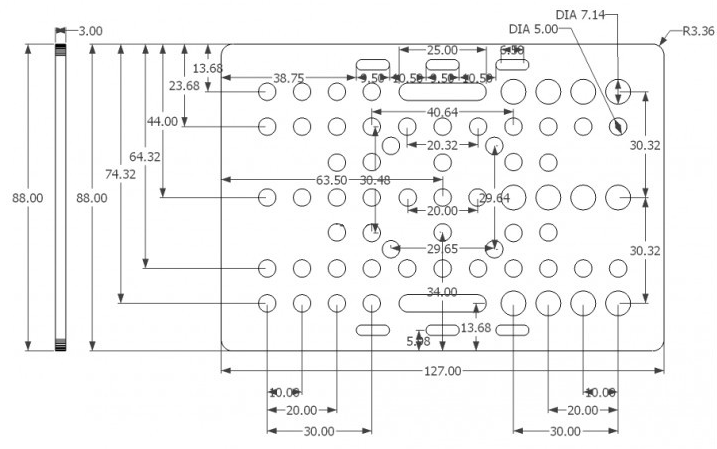
\includegraphics[width=\textwidth]{construct_gantry-plate.png}%
    \end{center}

    \fullcite{carew:gantry-plate-schematic}
\end{figure}

Ορισμένες οπές είναι διαμέτρου 7.14mm και βρίσκονται συγκεντρωμένες στο δεξί
μισό του σχήματος.
Οι συγκεκριμένες χρησιμοποιούνται σε συνδυασμό με έκκεντρα διαχωριστικά έναντι
απλών (σχήμα \ref{fig:construct:wheel_exploded}γ) των οποίων η προεξοχή
εισέρχεται στην οπή. Περιστρέφοντας τους, μεταβάλλεται η απόσταση των
αντίστοιχων τροχών από τον οδηγό έως ότου εφάπτονται ερμητικά με την αυλάκωση
ώστε να αποφεύγονται οι κραδασμοί κατά την κίνηση της πλάκας.
Τοποθετώντας τροχούς σε κατάλληλα ζεύγη οπών 5 και 7.14mm δημιουργείται διάκενο
στο οποίο εισέρχεται οποιοδήποτε από τα τέσσερα μεγέθη οδηγών.

%\section{Γραμμική κίνηση}

Μετάδοση κίνησης

\section{Βάση}

\label{sec:construct:base}
Η βάση της συσκευής αποτελείται από πλαίσιο κατασκευασμένο από παραλληλεπίπεδους
οδηγούς, αναρτημένο σε τέσσερις γωνιακούς οδηγούς στήριξης. Η συγκράτηση των
οδηγών επιτυγχάνεται με χρήση γωνιακών προσαρτημάτων, κοχλιών M5 και περικοχλίων
ένθετων στις αυλακώσεις των οδηγών (σχήμα \ref{fig:construct:base}). Όπως
γίνεται αντιληπτό, στοιχεία όπως κοχλίες, περικόχλια, αντιπερικόχλια, δακτύλιοι
\etc είναι απαραίτητα σε κάθε στάδιο της κατασκευής. Ωστόσο, σημειώνεται ότι
αποφεύγεται η τόσο λεπτομερής ανάδειξη των επιμέρους αυτών στοιχείων, εφόσον
κρίνεται ότι στερούνται ουσιαστικού ενδιαφέροντος.

Στον κενό χώρο που σχηματίζεται κάτω από το πλαίσιο, τοποθετείται το δοχείο
παρακολούθησης το οποίο και τον καλύπτει χωρίς, ωστόσο, να εισέρχεται στο
πλαίσιο. Ο χώρος του πλαισίου αφιερώνεται, εξ ολοκλήρου, στην κίνηση των οργάνων
της συσκευής και είναι απαραίτητο να παραμένει ελεύθερος από εμπόδια. Αυτός
είναι και ο λόγος που έχουν επιλεγεί για το πλαίσιο οι τόσο πλατιοί οδηγοί των
8cm· ώστε να καλύπτονται επαρκώς τα κινητά του όργανα καθώς και να παρέχεται ένα
εύληπτο όριο για το ύψος του δοχείου. Περισσότερες λεπτομέρειες σχετικά με τα
κινητά όργανα που προστατεύονται από το πλαίσιο δίνονται στην
\ref{sec:construct:z-axis}.

Το ύψος της βάσης και, συνεπώς, του δοχείου, περιορίζεται από το μέγεθος των
ίδιων των αισθητήριων οργάνων καθώς θα ήταν άσκοπο έως και επιβαρυντικό για την
εξαγωγή έγκυρων μετρήσεων, εάν υπάρχει βάθος στο δοχείο το οποίο παραμένει
απροσπέλαστο από τους αισθητήρες και αδύνατο να καταμετρηθεί.
Δεδομένου ότι οι επιλεγμένοι αισθητήρες υγρασίας και οξύτητας έχουν μήκος
περίπου 21cm, για τη στήριξη του πλαισίου επιλέγονται οδηγοί 30cm, 8cm των
οποίων χρησιμοποιούνται για την προσάρτησή τους στο πλαίσιο (σχήμα
\ref{fig:construct:base}).

Οι άλλες δύο διαστάσεις είναι σχεδόν ανεξάρτητες με τους μοναδικούς περιορισμούς
να τίθενται σχεδόν κατά αποκλειστικότητα από τις δυνατότητες του
μικροεπεξεργαστή καθώς και από πρακτικούς λόγους όπως το μέγεθος της επιφάνειας
προς διαχείριση.
Ωστόσο, επειδή έχει γίνει ήδη αναφορά στο μέγεθος του δοχείου σε σχέση με τη
βάση, σημειώνεται ότι η υπό παρακολούθηση περιοχή είναι ελαφρώς μικρότερη από
τις πραγματικές εσωτερικές διαστάσεις του πλαισίου, επειδή δημιουργείται ένα
μικρό περιθώριο ως αποτέλεσμα της επιλεγμένης διάταξης των διαφόρων μηχανικών
στοιχείων.
Οι λόγοι ύπαρξης του περιθωρίου γίνονται περισσότερο αντιληπτοί στις επόμενες
ενότητες.

\begin{figure}
    \caption{Η βάση της συσκευής. \label{fig:construct:base}}
    \begin{center}%
    \def\svgwidth{\textwidth}
    \input{img/construct_base_exploded.pdf_tex}
    \end{center}
\end{figure}

\section{Άξονας Y}

Τροχοφόρος πλάκα τοποθετείται παράλληλα προς το έδαφος με τους τροχούς της στην
κορυφαία αυλάκωση ενός περιμετρικού οδηγού της βάσης. Στο σχήμα
\ref{fig:construct:belt-pulley-y} απεικονίζεται η βασική διάταξη των εξαρτημάτων
σε μία ενδεικτική απλοποιημένη υλοποίηση.
Στην εξωτερική πλευρά της πλάκας (α) βρίσκεται κινητήρας από τον οποίο
εκτείνεται ράβδος (β) που φέρει την κινητήρια τροχαλία (γ).
Τραπεζοειδής ιμάντας τεντωμένος κατά μήκος της εξωτερικής αυλάκωσης του οδηγού
και στερεωμένος στα άκρα του, αξιοποιεί τους τροχούς ως ελεύθερες τροχαλίες ώστε
να αυξάνεται το τόξο επαφής με την κινητήρια τροχαλία.

\begin{figure}
    \caption{Κινητή τροχαλία και ιμάντας. \label{fig:construct:belt-pulley-y}}
Διάταξη τροχαλίας-ιμάντα για την κίνηση στον άξονα Y. Ο κινητήρας έχει
αποκλειστεί από την απεικόνιση. Ωστόσο, νοείται ότι βρίσκεται συζευγμένος με τη
ράβδο (β) στο ελεύθερο άκρο της.
    \begin{center}%
    \def\svgwidth{0.7\textwidth}
    \input{img/construct_belt-pulley-y.pdf_tex}
    \end{center}
\end{figure}

\section{Άξονας X}

Σε αυτήν την πλάκα, στερεώνεται το ένα άκρο του γεφυρώματος, ένας νέου οδηγού ο
οποίος ενώνει αυτή με την απέναντι πλευρά της βάσης, πάνω στο οποίο εκτελείται η
κίνηση στον άξονα X.
Ωστόσο, επιλέγεται ελαφρώς διαφορετική προσέγγιση από αυτήν που χρησιμοποιήθηκε
για τον άξονα Y. Βασικό λόγο αποτελεί η τοποθέτηση του κινητήρα και αυτού του
άξονα στην ίδια πλάκα με αυτήν του κινητήρα του άξονα Y, προκειμένου η καλωδίωση
του να εκτείνεται προς ένα κινητό σημείο και όχι, δυνητικά, όλου του πλάτους της
βάσης. Επίσης, με αυτόν τον τρόπο αξιοποιείται μεγαλύτερο μέρος της επιφάνειας
της πλάκας γεφυρώματος.

Στο σχήμα \ref{fig:construct:x-axis-schem} παρουσιάζεται η υλοποίηση του άξονα
X.
Ο κινητήρας X τοποθετείται κοντά στο κέντρο της πλάκας γεφυρώματος (β) με τη
βάση της τροχαλίας (α) παράλληλα προς την πλάκα και ελαφρώς υψηλότερα της ώστε ο
ιμάντας να ευθυγραμμίζεται με αυλάκωση του γεφυρώματος. Η πλάκα φορτίου του
άξονα X τοποθετείται κάθετα ως προς το δάπεδο και ο ιμάντας προσδένεται στις
σχετικές πλαϊνές της οπές. Στην πλευρά της πλάκας πλησιέστερη της τροχαλίας
(στ), ο ιμάντας προσδένεται απευθείας, ενώ στην άλλη, εφόσον διανύσει το μήκος
του γεφυρώματος και αναστραφεί σε ελεύθερη τροχαλία (η) στο άλλο άκρο του.

Στο άκρο της ελεύθερης τροχαλίας, επιλέγεται διαφορετικός τρόπος στερέωσης και
ανύψωσης του οδηγού από τη βάση. Ουσιαστικά, απαλείφεται η πλάκα γεφυρώματος και
χρησιμοποιούνται δύο τροχοί αντί τεσσάρων, οι οποίοι στερεώνονται απευθείας στον
οδηγό. Ο βασικότερος λόγος είναι η αξιοποίηση μεγαλύτερου μήκους του οδηγού,
καθώς μία πλάκα γεφυρώματος, συνολικού μήκους 12.7cm, επιφέρει μεγαλύτερο
περιθώριο (θ) εσωτερικά της βάσης από ότι ένας τροχός. Η επιλογή αυτή
ενδυναμώνεται περαιτέρω από το γεγονός ότι μία πλάκα στο σημείο αυτό θα
χρησιμοποιούταν μόνο για τους τροχούς και την ελεύθερη τροχαλία.

Ωστόσο, παραμένει βασική προϋπόθεση η χρήση κάποιου εξαρτήματος στη θέση της
πλάκας που έχει το ίδιο πάχος, ώστε να διατηρείται οριζόντιος ο οδηγός. Το
μικρότερο εξάρτημα που εντοπίστηκε είναι το πώμα (ζ) το οποίο, τυπικά,
προορίζεται για την κάλυψη των άκρων των οδηγών. Η ορατή έδρα του στο σχήμα, η
οποία διαθέτει μία κοιλότητα, εφάπτεται στον οδηγό. Η άλλη έδρα είναι πλήρως
επίπεδη και σε αυτήν ακουμπά το διαχωριστικό. Επομένως, δεδομένου ότι
χρησιμοποιούνται διαχωριστικά (δ) και επίσωτρα (γ) ίδιου ύψους, ο οδηγός
διατηρείται οριζόντιος.

\begin{figure}
    \caption{Συστατικά μέρη γεφυρώματος. \label{fig:construct:x-axis-schem}}
    \begin{center}%
    \def\svgwidth{\textwidth}
    \input{img/construct_x-axis.pdf_tex}
    \end{center}
\end{figure}

Η ελεύθερη τροχαλία δημιουργείται με επίσωτρο που παρέχει το σύστημα κατασκευής
με τρόπο αντίστοιχο αυτού της σύνθεσης των τροχών. Συνεπώς, ελεύθερες τροχαλίες
μπορούν να τοποθετηθούν απευθείας σε αυλακώσεις οδηγών ή σε πλάκες γεφυρώματος.
Επίσης, παρέχεται και μία διαφορετική μικρότερη πλάκα με λιγότερες οπές ειδικά
για αυτόν το σκοπό (απεικονιζόμενη στο σχήμα \ref{fig:construct:x-axis-schem}η).

Απευθείας προσάρτηση της ελεύθερης τροχαλίας σε αυλάκωση του οδηγού αποκλείεται
σε αυτήν την περίπτωση, καθώς οι διαθέσιμες αυλακώσεις καθιστούν αδύνατη την
άμεση επικοινωνία της με την κινητήρια τροχαλία. Εφόσον έχει ήδη αποκλειστεί η
χρήση πλάκας γεφυρώματος για την αποφυγή άσκοπης σπατάλης χώρου, επιλέγεται η
προσάρτηση της ελεύθερης τροχαλίας στην ειδική πλάκα και, μέσω αυτής, είτε στην
επάνω αυλάκωση του οδηγού (όπως και στο σχήμα \ref{fig:construct:x-axis-schem}),
είτε, εναλλακτικά, στην κάτω αυλάκωση, αντικαθιστώντας το εξωτερικό πώμα.

\section{Άξονας Z}

\label{sec:construct:z-axis}
Τελικά, στην πλάκα φορτίου του άξονα X στερεώνεται το κατώτερο τμήμα οδηγού για
την κίνηση στον άξονα Z, με το μεγαλύτερο τμήμα του να εκτείνεται πάνω από την
πλάκα. Και σε αυτήν την περίπτωση επιλέγεται η χρήση ιμάντα σε συνδυασμό με
κινητήρια και ελεύθερη τροχαλία. Επειδή ενδιαφέρει η μετακίνηση μόνο των
αισθητήρων που προορίζονται για την παρακολούθηση του υλικού, επιλέγεται η πλάκα
Mini~V, η οποία χαρακτηρίζεται από πολύ μικρό μέγεθος, και πάνω σε αυτήν
προσαρτώνται οι αισθητήρες, όπως φαίνεται αριστερά στο σχήμα
\ref{fig:construct:z-axis}. Η εμφανιζόμενη θήκη αποτελεί μέρος των προμηθευμένων
αισθητήρων υγρασίας και οξύτητας η οποία έχει τροποποιηθεί ώστε να στεγάζεται
ένας ακόμα αισθητήρας, αυτός της θερμοκρασίας (γ), και για τη δημιουργία
ορισμένων πρόσθετων οπών για τους κοχλίες και τις γραμμές σήματος.

\begin{figure}
    \caption{Αναπαράσταση οδηγού άξονα Z. \label{fig:construct:z-axis}}
Το μήκος του οδηγού είναι ενδεικτικό και όχι αντιπροσωπευτικό του πραγματικού.
Σημειώνεται ότι στο σχήμα δεξιά εμφανίζεται η διατομή ορισμένων στοιχείων.
    \begin{center}%
    \def\svgwidth{0.5\textwidth}
    \input{img/construct_z-axis.pdf_tex}
    \end{center}
\end{figure}

%belt path
Δεξιά του ίδιου σχήματος εμφανίζεται η διάταξη των στοιχείων που συνθέτουν τον
οδηγό Z. Όπως γίνεται αντιληπτό και από το σχήμα, οι βίδες και τα προσαρτήματα
για τη στερέωση του οδηγού που βρίσκονται χαμηλά στην οπίσθια αυλάκωσή του (α),
αποτρέπουν τη διέλευση του ιμάντα από αυτήν. Για το λόγο αυτό επιλέγεται οδηγός
VSlot~40 ώστε, εναλλακτικά της αυλάκωσης, να αφιερώνεται η ενδιάμεση σήραγγα ως
δίοδος επιστροφής του ιμάντα.

Όπως φαίνεται και στο σχήμα, η ελεύθερη τροχαλία στερεώνεται λίγο διαφορετικά σε
σχέση με τους τρόπους που έχουν προηγουμένως αναφερθεί, αντικαθιστώντας την
ειδική πλάκα με δύο απλά προσαρτήματα. Ο λόγος είναι η αξιοποίηση περισσότερου
μήκους των αισθητήρων, εφόσον τα απλά προσαρτήματα δεσμεύουν λιγότερο χώρο της
αυλάκωσης στην οποία κινείται και η πλάκα Mini~V με αποτέλεσμα, η τελευταία, να
μετακινείται χαμηλότερα στον άξονα Z.

Δεδομένου ότι η πλάκα φορτίου του άξονα X (β) εκτείνεται κάτω από τον οδηγό της,
πρέπει να εξασφαλίζεται ότι και αυτή καθώς και τα υπόλοιπα μέρη, κινούνται χωρίς
να παρεμποδίζονται από τρίτα αντικείμενα. Αυτό αιτιολογεί τη χρήση αρκετά πλατύ
οδηγού για το πλαίσιο της βάσης, όπως αναφέρεται στην ενότητα
\ref{sec:construct:base}.
%Έχει σημειωθεί σε προηγούμενη ενότητα ότι το πλαίσιο της βάσης της συσκευής
%χρησιμοποιείται σαν προστατευτικό για τα κινητά μέρη της συσκευής και
%αποφεύγεται να εισέρχονται εμπόδια σε αυτό. Το κομμάτι
%που προστατεύεται με αυτόν τον τρόπο είναι 
%
%Servo VS Stepper ~~!!

\section{Τοποθέτηση κινητήρων}

Ενώ το σύστημα κατασκευής OpenBuilds παρέχει πολλά εξαρτήματα για την κάλυψη
πληθώρας αναγκών, έχει, ωστόσο, αποβεί αδύνατος ο εντοπισμός κάποιων που να
διευκολύνουν την τοποθέτηση κινητήρων servo. Αντιθέτως, το σύστημα Actobotics
είναι προσανατολισμένο προς τέτοιους κινητήρες. Μολονότι τα δύο συστήματα
παρουσιάζουν χαμηλή συμβατότητα στα εξαρτήματά τους, μπορούν να συνυπάρξουν, έως
ένα βαθμό.
% ως άμεση απόρροια χρήσης %διαφορετικού Συστήματος Μονάδων, μελετήθηκε και εντοπίστηκε ότι είναι δυνατό να
%>> λόγω διαφορετικής διάταξης των οπών τους

\begin{figure}
    \caption{Κανάλι Actobotics και διάταξη οπών.
        \label{fig:construct:acto-channel-pattern}}
    \begin{center}
        \begin{subfigure}[b]{0.40\textwidth}
            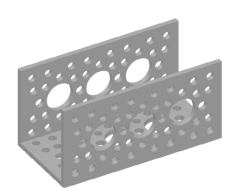
\includegraphics[width=0.95\textwidth]{construct_acto-channel-3in.png}
            \caption{}
        \end{subfigure}
        \begin{subfigure}[b]{0.35\textwidth}
            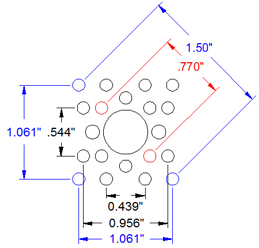
\includegraphics[width=0.9\textwidth]{construct_acto-pattern.png}
            \caption{}
        \end{subfigure}
    \end{center}

    (βʹ): \fullcite{actobotics:channel-pattern}
\end{figure}

Η λύση εντοπίζεται στις κυκλικά διατεταγμένες οπές των καναλιών -- αντίστοιχων
μονάδων των οδηγών VSlot -- οι οποίες απέχουν 0.77in, περίπου 2cm, (σχήμα
\ref{fig:construct:acto-channel-pattern}β), δηλαδή όσο και οι οπές πλακών και
περικοχλίων του OpenBuilds, με αποτέλεσμα να μπορούν να συνδεθούν στα σημεία
αυτά.
Επομένως, επιλέγεται να χρησιμοποιηθούν εξαρτήματα Actobotics για την πλαισίωση
των κινητήρων και, ως βάση, το κανάλι του εν λόγω συστήματος το οποίο στη
συνέχεια προσδένεται σε κάποιο εξάρτημα του συστήματος OpenBuilds. Στην
περίπτωση του κινητήρα Z, το κανάλι προσδένεται απευθείας σε αυλάκωση του 
αντίστοιχου οδηγού ενώ στην περίπτωση των X και Y, πάνω στην πλάκα γεφυρώματος.

Μία κατηγορία εξαρτημάτων του συστήματος Actobotics ιδιαίτερου ενδιαφέροντος
είναι τα στηρίγματα κινητήρα, τα οποία επιτρέπουν πολλές και σύνθετες διατάξεις
τους. Μολονότι παρέχεται στήριγμα που στερεώνεται απευθείας στις γωνιακές οπές
του καναλιού, επιλέγεται στήριγμα που απαιτεί πρόσθετα γωνιακά προσαρτήματα ώστε
ο κινητήρας να εξωθείται ελαφρώς υψηλότερα από το κανάλι προκειμένου να
αξιοποιείται κατά το μέγιστο δυνατό ο χώρος στο εσωτερικό του καναλιού.
Η ανάγκη αυτή προκύπτει για τον κινητήρα του άξονα X όπου η τροχαλία βρίσκεται
στο εσωτερικό του καναλιού. Για περισσότερη ομοιομορφία μεταξύ των κινητήρων,
επιλέγεται η ίδια διάταξη για όλους, παρότι δεν υφίσταται αντίστοιχη επιτακτική
ανάγκη.

\begin{figure}
    \caption{Διάταξη κινητήρων αξόνων X και Y.\label{fig:construct:xy-servo}}
    \begin{center}%
    \def\svgwidth{0.5\textwidth}
%    \input{img/construct_xy-servo.pdf_tex}
    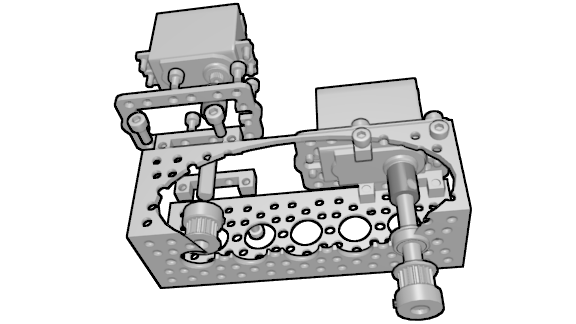
\includegraphics[width=\textwidth]{construct_xy-servo.png}
    \end{center}
\end{figure}
%
%Επιλέγονται γωνιακά προσαρτήματα για την εξώθηση του στηρίγματος του κινητήρα
%ελαφρώς υψηλότερα από το κανάλι ώστε να αξιοποιείται κατά το μέγιστο δυνατό ο
%χώρος στο εσωτερικό του. Η ανάγκη αυτή προκύπτει για τον κινητήρα του άξονα X
%όπου η τροχαλία βρίσκεται στο εσωτερικό του καναλιού. Για περισσότερη
%ομοιομορφία μεταξύ των κινητήρων, επιλέγεται η ίδια διάταξη για όλους, παρότι
%δεν υφίσταται αντίστοιχη επιτακτική ανάγκη.

Στο σχήμα \ref{fig:construct:xy-servo} παρουσιάζεται η διάταξη των στοιχείων για
τους κινητήρες των αξόνων X και Y.
Στην άτρακτο του κινητήρα προσαρτάται σύνδεσμος και, δια μέσω αυτού, το ένα άκρο
ράβδου περιστροφής. Για τους κινητήρες X και Z, η ράβδος είναι αρκετά μακρυά
ώστε να διέρχεται από ένσφαιρο τριβέα τοποθετημένο σε οπή 0.5in του καναλιού. Ο
επιπρόσθετος τριβέας αυξάνει την σταθερότητα της ράβδου, ιδίως όταν στα άκρα της
εφαρμόζεται ακτινικό φορτίο (μέσω του ιμάντα).

Η διατομή της ράβδου είναι σχήματος D και όχι κυκλική ώστε να δημιουργείται μία
επίπεδη επιφάνεια η οποία εξυπηρετεί την ασφαλέστερη πρόσδεση εξαρτημάτων που
διαθέτουν ένθετο κοχλία σύσφιξης. Τόσο ο σύνδεσμος όσο και η κινητήρια τροχαλία
επωφελούνται από αυτήν την ιδιότητα της ράβδου.

\begin{figure}
    \caption{Αναπαράσταση της συσκευής.}
    \begin{center}%
%    \def\svgwidth{0.6\textwidth}
    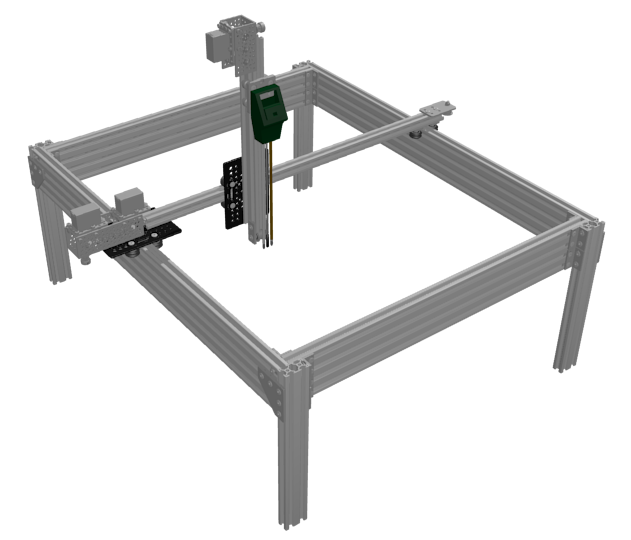
\includegraphics[width=\textwidth]{construct_device.png}
    \end{center}
\end{figure}
